

\chapter[Repères historiques]{Repères historiques et religions de la péninsule arabique à l'aube du VII\textsuperscript{e} siècle}


\textbf{Objectifs}

\begin{itemize}
\item
  Se repérer dans l'histoire des premiers siècles de l'islam
\item
  Origine du mot «~arabe~».
\item
  Les prismes méthodologiques de l'historiographie musulmane
\item
  Panorama religieux de l'Arabie
\item
  Saisir l'existence d'un judaïsme et d'un christianisme spécifiques à
  cette région à la veille de la prédication de Muḥammad.
\item
  Articulation et interactions des religions (judaïsme, christianisme,
  manichéisme\ldots) sur les rites et croyances musulmanes
\end{itemize}


\vide{pruxe9ambule}{%
\section{Préambule}\label{pruxe9ambule}}

Un cours sur les fondations de l'islam s'intéresse donc aux fondations,
c'est-à-dire aux bases, aux fondements, aux piliers de l'islam. Nous les
traiterons. Mais ces pratiques musulmanes d'où viennent-elles~? Question
à laquelle on peut reprocher de s'inscrire dans une approche
historico-critique, celle des orientalistes pris entre deux feux, celui
de l'idéalisation de l'islam et son aversion, entre sa «~fascination~»
pour reprendre l'expression de Maxime Rodinson et sa répulsion. Poser
une lecture historico-critique dont la méthode et la démarche émanent du
monde occidental, ne serait-il pas imposé à l'islam une compréhension et
une lecture qui ne sont pas celles de son univers théologique~? Pour des
chercheurs philosophes ou historiens tels Mohammad Arkoun ou Abdesselam
Cheddadi, il importe de situer l'histoire de l'islam dans son contexte
historique et d'explorer cet univers religieux où l'islam est né. À cet
égard, si pour Henri Pirenne, l'avènement de l'islam a constitué une
rupture radicale et irrévocable dans la civilisation méditerranéenne,
Cheddadi montre au contraire, la continuité avec la tradition de
l'Antiquité tardive.

Pour autant, les lectures historiques ne sont pas sans limites et
défauts. Rappelez-vous la bibliographie générale. À propos de
l'orientaliste Maxime Rodinson, j'indiquais qu'il avait étudié l'islam
en prenant comme grille de lecture la pensée marxiste~: pour lui, on ne
peut comprendre l'essor d'une religion qu'en lien avec
«~l'infrastructure~», donc en l'occurrence en lien avec l'environnement
socio-économico-politique de la péninsule arabe, et donc de La Mecque et
de Médine. Sans épouser forcément la lecture marxiste de l'histoire, il
est certain que «~l'islam n'est pas tombé du ciel~». Or, cette
affirmation ne saurait être contraire à la foi musulmane. Certes, la
recherche scientifique sur le Coran peut être troublante et paraître
s'opposer au dogme du Coran incréé, mais pour ce qui est de l'islam, il
y a forcément une histoire, un contexte culturel, un jeu d'interactions
multiples dans lequel il a pris naissance. Ces contextes sont attestés
par les historiens musulmans eux-mêmes, qui tout au long des premiers
siècles de l'islam ont écrit une historiographie islamique. Que
d'informations minutieuses ne sont par eux rassemblées, qu'il s'agisse
de Ibn Qutayba (m. 889)\sn{On évitera de mettre une croix pour
  signaler la date de la mort d'un auteur musulmans~: m. renvoie à la
  date de sa mort. Si nous mettons deux dates séparées par un oblique,
  la première renvoie au calendrier hégirien (H 0 = 622), la seconde au
  calendrier romain. S'il n'y a qu'une date, c'est toujours le
  calendrier romain.} ou d'a-Mas'ūdī (m. 956) dans son ouvrage \emph{Les
prairies d'or} ! Mais l'histoire comme science a développé une
méthodologie critique~; elle souligne le travail de reconstruction
propre aux historiens à la lumière des questions et de l'environnement
socio-politique dans lequel ils travaillent. Quand émerge une nouvelle
dynastie, comme c'est le cas avec les Abbasides qui succèdent aux
Omeyyades et qui vont régner de 750 à 1258, évidemment, on réécrit
l'histoire et on gomme certains événements historiques pour plaire aux
nouveaux princes et asseoir la légitimité de leur pouvoir dans
l'histoire. C'est vieux comme Hérode. Le mécanisme est mis en lumière
par Orwell dans \emph{1984~}avec le fameux bureau de la falsification
historique où l'histoire est reconstruite en fonction des alliances
politiques~: il s'agit d'effacer les preuves~que l'histoire s'est passée
comme elle s'est passée~! Même exemple de falsification historique sur
les photos de Lénine, où Staline a fait effacer Trotski\ldots{} 

\vide{i--la-puxe9ninsule-arabique-terreau-de-la-pruxe9dication-de-muux1e25ammad}{%
\subsection{{La péninsule arabique, terreau de la
prédication de Muḥammad
}}\label{i--la-puxe9ninsule-arabique-terreau-de-la-pruxe9dication-de-muux1e25ammad}}

La question est donc de savoir ce qu'est l'Arabie à la veille de la
naissance de l'islam~: une vaste péninsule située au sud-ouest de
l'Asie, à la jonction entre ce continent et l'Afrique. On distingue
l'Arabie déserte, l'Arabie heureuse (Arabie du sud, l'actuel Yémen --
Arabie humide, grâce aux montagnes), l'Arabie pétrée (province romaine
d'Arabie créée en 106 après la conquête du royaume nabatéen et ayant
pour capitale Pétra). L'Arabie déserte est habitée par un peuple de
bédouins dont la culture est celle des tribus. Regardons de plus prêt.
Vérifions. Mais au préalable, comment savoir~? Sur quelles sources
s'appuyer~?

\vide{la-question-des-sources-historiques}{%
\subsubsection{La question des sources
historiques}\label{la-question-des-sources-historiques}}

L'historiographie musulmane, disions-nous, n'échappe pas au travers de
la reconstruction historique. Mais que dit-elle~?

\vide{la-tradition-de-lhistoriographie-musulmane-entre-ux1e7ux101hiliyya-et-muux2bfallaqux101t}{%
\paragraph{{1.1.1 La tradition de l'historiographie
musulmane~: entre ǧāhiliyya et muʿallaqāt
}{1.1.1 La tradition de l'historiographie musulmane~: entre ǧāhiliyya et muʿallaqāt }}\label{la-tradition-de-lhistoriographie-musulmane-entre-ux1e7ux101hiliyya-et-muux2bfallaqux101t}}

En général, les historiens musulmans voient dans les temps qui précèdent
l'islam un moment de profonde anarchie. Il s'agit par contraste de faire
ressortir ce qu'a apporté l'islam. Ainsi, l'Arabie antéislamique est
marquée par la \emph{\textbf{ğāhiliyya}}, c'est-à-dire l'ignorance des
lois de la révélation. Retenez ce terme\ldots{} on le retrouve sous la
plume des grands théoriciens du vingtième siècle de l'islam politique à
l'exemple de Sayyid Quṭb, un frère musulman égyptien à l'influence
considérable ou de Mawdudi (on a déjà parlé de ce dernier dans
l'introduction. De quelle nationalité est-il~? Réponse dans le chapitre
précédent si besoin était). Tous deux parlent du monde moderne comme
d'une seconde \emph{ğāhiliyya}. Les tribus sont querelleuses comme
l'attestent les poèmes de la période, il n'y a pas d'État, pas d'ordre,
pas de sécurité, pas de paix. On pratique la \emph{razzia} et les
\emph{pillages}. Bref, c'est le chaos.

La situation économique est précaire. La Mecque connaît souvent la
famine. Et selon la tradition arabo-musulmane, alors qu'il fallait
reconstruire le sanctuaire de la Ka`ba, le bois manquant, il fallut
recourir pour les poutres, au bois de l'épave d'un navire byzantin ayant
échoué\sn{\textsuperscript{~}Christian Robin, «~La péninsule
  Arabique à la veille de la prédication muhammadienne~», dans Thierry
  Bianquis, Pierre Guichard, Mathieu Tillier, \emph{Les débuts du monde
  musulman, VIIe-Xe siècle}, Nouvelle Clio, Paris, PUF, 2012, p. 6.}.
Sur le plan de la culture, la \emph{ǧāhiliyya} est aussi marquée par
l'illettrisme et une certaine déchéance religieuse, le désordre des
cultes multiples.

Qu'en est-il de cette description~historique ? Remarquons que les
razzias sont, pour ces populations, vitales. Elles n'ont pas le choix à
moins de quitter le désert. On n'attaquait pas une caravane par plaisir
ou par brutalité, mais par nécessité pour vivre. Par ailleurs, l'idée
d'une ignorance culturelle est difficilement compatible avec la riche
tradition poétique antéislamique qu'on appelle les
\emph{mu`allaqāt}\sn{Charles Pellat,~\emph{Langue et littérature
  arabes}, Paris, 1970. Les \emph{mu`allaqāt} sont des odes
  préislamiques. Voir~: \emph{Les Suspendues (Al-Mu'allaqât)}, trad. et
  prés. par Heidi TOELLE, éd. Flammarion coll. GF, Paris, 2009 et Pierre
  Larcher, \emph{Le brigand et l'amant, deux poèmes préislamiques de
  Ta'abbata Sharran et Imru' al-Qays,} traduits de l'arabe et commentés,
  suivis des adaptations de Goethe et d'Armand Robin et de deux études
  sur celles-ci, Sindbad, Actes Sud, 2012 et Pierre Larcher, \emph{Les
  Mu'allaqât, les sept poèmes préislamique,} traduits et commentés, Fata
  Morgana, 2000.} et qui est elle-même reconnue par la tradition
musulmane. Ces poèmes ne sont pas `barbares'~; leur expression, leur
rythmique, leur métrique témoignent d'une langue raffinée. Chefs d'œuvre
de la littérature arabe anté-islamique, ils sont particulièrement
importants pour saisir un univers religieux, symbolique, spirituel, des
modes de vie, des us et coutumes, des rites, mais aussi l'âme de ces
poètes, leur imaginaire, leurs désirs~; Il va être forcément question
d'amour, mais la manière dont ils en parlent permet de rejoindre leur
univers, celui d'hommes du désert en quête d'un point d'eau et de verts
pâturages.

\vide{section-1}{%
\subsubsection{}\label{section-1}}


\mn{Ici, vous trouverez l'émission Cultures
d'islam avec Pierre Larcher à l'occasion de la publication \emph{Le
brigand et l'amant.} Poeme connu depuis très longtemps avant
Goethe.}

Que nous disent ces poèmes~?

D'abord un mot sur le sens de ce terme : Il vient de la racine
\emph{`allaqa}, suspendre et viendrait de ces bijoux suspendus à une
chaîne et qui orneraient le temple de la Ka'ba.

L'univers géographique est celui d'un très vaste territoire~: l'Arabie,
ce n'est pas un désert, mais des déserts. Il y a des déserts de roche,
des déserts de sable dont certaines dunes s'élèvent à plus de 200m, des
déserts recouverts d'une fine végétation. Le climat est celui du feu et
il n'est pas rare que les températures atteignent 50° à l'ombre. En
hiver et au printemps des fortes pluies souvent dévastatrices font
refleurir le désert pour un temps éphémère. Des puits d'eau, des
rivières souterraines parsèment le territoire d'oasis.

Les bédouins sont des pasteurs nomades, sans cesse contraint de se
déplacer par tribu. On est dans un milieu tribal où l'on se revendique
d'une généalogie. \textbf{La tribu doit rester unie~: c'est une question
de vie}. La \emph{Muʿallaqa} de T'arafa Ibn al-ʿAbd expose un rebelle
qui est pour un temps exclu des siens. À la tête de chaque tribu on
trouve un conseil (\emph{mala'}) à qui il revient de discuter des
questions relatives aux affaires de la tribu~: alliances, combats,
guerres, négociations de paix, etc.

Socialement, le patriarcat domine~; mais les femmes disposaient d'une
certaine liberté~; elles pouvaient répudier leurs époux. Si un fugitif
trouvait asile sous une de leurs tentes il n'avait plus rien à craindre
de ses ennemis. Dans les guerres, une tribu peut demander la protection
d'une autre tribu plus puissante.

Certaines tribus sont parvenues à fonder des royaumes. On dénombre trois
dynasties~: les \textbf{lakhmides, les Ghassānides et les Kinda}. On
leur doit d'avoir contribué à la propagation d'une langue commune.
Certains de ces poèmes font mention de ces dynasties et aux guerres qui
ont pu les opposer.

Des us et coutumes, il est question du temple de la Ka`ba. Il y avait un
pèlerinage à La Mecque, il y avait le rite de la circumambulation de la
Pierre noire, la course entre les deux collines d'al-Sa'fā et
al-Marwa\ldots{} tout cela fait partie aujourd'hui du pèlerinage
islamique.

Dans le Panthéon arabe, il y avait un Dieu du nom d'Allāh et qui avait
trois filles~: al-Lāt, Manāt et al-ʿUzza (on les trouve mentionnée dans
le Coran~: S. 53 la liminaire , 19-20).

\begin{table}[h!]
    \centering
    \small
   \begin{tabular}{p{0.45\textwidth}p{0.45\textwidth}}
\toprule
C'est alors que Dieu révéla à Son Serviteur ce qu'Il voulait lui
révéler. & Faawha ila AAabdihi ma awha (⁎) \\
53. 11 Et le cœur ne saurait démentir ce que les yeux ont vu. & Ma
kathaba alfuadu ma raa (⁎) \\
Allez-vous donc lui contester ce qu'il a de ses propres yeux vu, &
Afatumaroonahu AAala ma yara (⁎) \\
53. 13 et alors qu'il l'avait déjà vu lors d'une précédente apparition,
& Walaqad raahu nazlatan okhra (⁎) \\
près du Lotus de la limite, & AAinda sidrati almuntaha (⁎) \\
non loin du Jardin du séjour des bienheureux, & AAindaha jannatu almawa
(⁎) \\
53. 16 au moment où un voile indéfinissable recouvrait le Lotus ? & Ith
yaghsha alssidrata ma yaghsha (⁎) \\
Le regard du Prophète n'a ni dévié ni outrepassé la mesure, & Ma zagha
albasaru wama tagha (⁎) \\
et c'est ainsi qu'il lui fut donné de voir certains des plus grands
signes de son Seigneur. & Laqad raa min ayati rabbihi alkubra (⁎) \\
19 Que pensez-vous cependant d'al-Lât, d'al-Uzzâ & Afaraaytumu allata
waalAAuzza (⁎) \\
et de Manât, cette autre troisième divinité ? & Wamanata alththalithata
alokhra (⁎) \\
53. 21 Auriez-vous ainsi des enfants mâles ; et Dieu, seulement des
filles ? & Alakumu alththakaru walahu alontha (⁎) \\
Ne voilà-t-il pas un partage des plus iniques ? & Tilka ithan qismatun
deeza (⁎) \\
En vérité, ce ne sont là que des noms que vous avez inventés, vous et
vos ancêtres, et que Dieu n'a investis d'aucune autorité. En réalité,
les idolâtres ne font que suivre leurs conjectures et leurs caprices,
alors que la bonne voie leur a bien été tracée par leur Seigneur. & In
hiya illa asmaon sammaytumooha antum waabaokum ma anzala Allahu biha min
sultanin in yattabiAAoona illa alththanna wama tahwa alanfusu walaqad
jaahum min rabbihimu alhuda (⁎) \\
\bottomrule
\end{tabular}
\sidecaption{S. 53 la liminaire , 19-20}
\end{table}

Il y a un dieu du soleil un dieu de l'orage, ainsi que des esprits
maléfiques. Chose étrange, le seul nom de Dieu qui est évoqué dans les
\emph{Muʿallaqāt} est Allāh. Les dieux ont-ils été expurgés, oubliés~?
Il reste que les rites eux sont bien mentionnés.

Les \emph{Muʿallaqāt} de Zuhayr rappellent que l'année était divisée
entre les mois profanes et les mois sacrés. Durant les mois sacrés, la
guerre est interdite~; le port des armes est prohibé dans les
sanctuaires.

Parmi les rites, la vengeance (\emph{tha'r}) en cas de meurtre avec le
risque de machine infernale. Pour l'éviter, on pouvait payer le prix du
sang qui s'élevait parfois à des milliers de chamelle. Tant que la
vengeance n'est pas accomplie, le vengeur devait subir des privations,
ne pas se couper les cheveux, ne pas se parfumer, de pas boire du vin,
ni avoir de rapports avec une femme. D'après un poème, on considérait
que la victime restait morte tant qu'elle n'était pas vengée ce qui
suggère une foi dans l'au-delà. On voit aussi une chamelle qu'on laisse
mourir sur la tombe de son maître suggérant la croyance que l'homme
avait besoin de sa chamelle dans l'autre vie.

Des combats, il nous est dit qu'ils avaient lieu à cheval~; on se
servait comme armes de la lance, des flèches, du sabre. Mais on essayait
de tuer le moins possible~: on cherchait avant tout à faire des
prisonniers qui pouvaient ainsi être échangés après des négociations.
Les razzias consistaient à surprendre une tribu à l'aube.

Le vin est chanté car il est aimé parmi les vaillants guerriers. Il
venait souvent de Syrie ou des vallées du Liban, de l'Euphrate ou de
l'Egypte~: il était souvent vendu par des marchands juifs ou chrétiens.

Dans ces poèmes se voit chanter deux chefs qui ont su mettre fin à
quarante ans de guerre. Le poète chante leurs louanges, leur magnanimité
et fustige tous les fauteurs de trouble qui ont envenimés un conflit
coûteux en vie.

À noter cependant que l'écrivain égyptien Taha Hussein (1889-1973) dans
son livre \emph{Fī al-ši`r al-ǧāhili} (1927) {[}De la poésie
préislamique{]} a remis en question l'authenticité de cette poésie~:
parce que fondée sur la tradition orale, en l'absence de documents
écrits, on ne peut être assuré de son authenticité. La thèse fit
scandale. D'une certaine manière, elle pouvait servir les partisans
d'une vision dichotomique entre le temps de l'ignorance et le temps de
l'islam. Mais elle heurta le public par le travail de déconstruction
qu'il y menait. On l'accusa d'apostasie.

Si la tradition musulmane a retenu les difficultés économiques qui ont
marqué la péninsule arabique au cours des 60-70 ans qui précèdent
l'avènement de l'islam, elle omet toute l'histoire des royaumes de
l'Arabie, histoire marquée par une grande stabilité et une richesse
économique, mais elle ne retient rien non plus de la présence des
monothéismes. Or, comment être sûr~de cette présence et de ces richesses
antérieures ? Grâce aux recherches archéologiques notamment.

\vide{les-recherches-archuxe9ologiques}{%
\subsubsection{{Les recherches archéologiques
}}\label{les-recherches-archuxe9ologiques}}

Dans le nord du Ḥiǧāz (région ouest de l'actuelle Arabie saoudite), en
Arabie du Sud-ouest, on trouve les vestiges de grandes villes antiques
avec des monuments, des œuvres d'orfèvrerie, des statues, des
sanctuaires, mais aussi des barrages hydrauliques. On peut citer parmi
les sites faisant l'objet d'investigations actuelles l'oasis d'al-`Ulā,
capitale d'un petit royaume appelé Dédān et qui a disparu au début de
l'ère chrétienne~; l'oasis de Taymā'~; le site de Madā'in Sālih
(l'antique Hijrā') où l'on trouve de magnifiques façades sculptées.

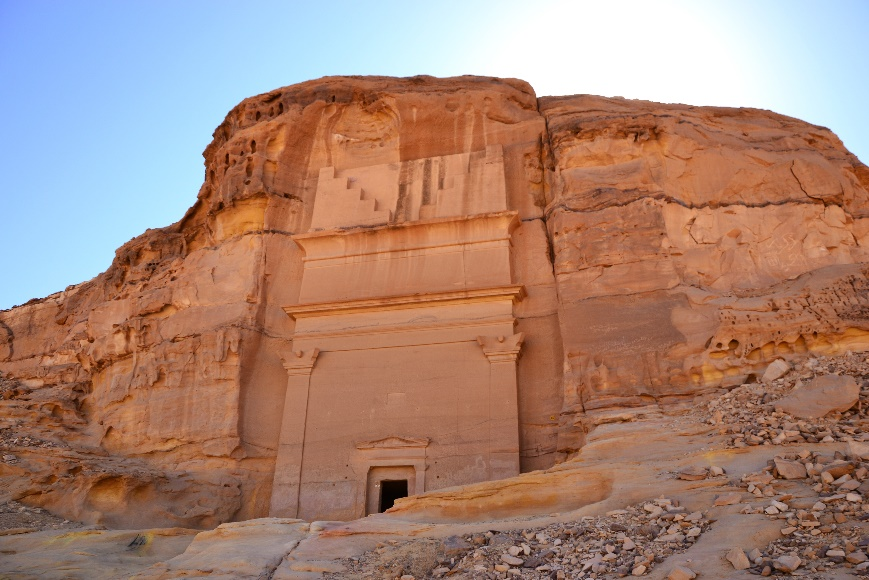
\includegraphics[width=3.94921in,height=2.63264in]{Images/image028.jpg}

Elle devient déserte à partir du IVe siècle et le Coran en donne la
raison~- Dieu a anéanti la ville, parce que ses habitants n'ont pas cru
aux prophètes~:
\begin{quote}
    «~Certes, les Hommes d'al-Hijr ont traité les Envoyés d'imposteurs. Nous
leur avons apporté Nos signes et ils se sont détournés. Ils creusèrent,
tranquilles, des demeures dans les montagnes. Mais le Cri les prit au
matin, et à rien ne leur servit ce qu'ils possédaient~» (S. 15,
80-84)\sn{\textsuperscript{~}S.~15, 80-84 signifie que ce sont les
  versets 80 à 84 de la sourate 15\ldots{} on y reviendra dans le
  chapitre sur le Coran.}.
\end{quote}



\begin{Synthesis}
Le Coran donne des informations
historiques, sur des épisodes passés, mais aussi sur l'histoire à
venir~. Mais il donne
surtout une lecture théologique de l'histoire.
\end{Synthesis}

Notons aussi l'existence de villes. \mn{La ville de Najran avait un évêque qui était probablement rattaché à l'église d'Éthiopie. Dhu Nuwas haïssait les chrétiens et faisait sans cesse la guerre au roi d'Éthiopie. Vaincu et forcé de payer tribut à Elesbaan, il se vengea sur les chrétiens de son royaume. Il agit par ruse : ayant rendu une visite protocolaire à la ville de Najran, il invita les notables à venir le voir dans son camp où ils furent tous capturés.   Devant leur refus de devenir juif, il
fait exécuter les 340 chrétiens de la ville, et décapiter le prince
Aréthas. Suite à ce massacre, le roi d'Ethiopie Elesbaan mena une
expédition punitive dans la cité, chassant Dounass, et rétablissant un
prince chrétien à la tête de la cité. Selon la plupart des commentateurs
du Coran, les hommes de Ukhdoud mentionnés au verset 4 de la sourate 85
ne seraient autres que les martyrs de Najran, tués et
brûlés.}
Najrān est située en Arabie saoudite
à proximité du Yémen. Elle a été aussi capitale d'un petit royaume. Elle
était habitée par des juifs et des chrétiens. Un épisode terrible y a eu
lieu et est resté dans les esprits lorsque le roi juif Himyar en 523 a
fait assassiner des notables chrétiens.



Dans le Golfe et dans le Nord du Hijāz, les travaux archéologiques ont
mis en lumière des langues étrangères (akkadien, araméen, nabatéen,
grec, latin). Mais qu'en est-il de l'arabe comme idiome linguistique~?

\vide{lessor-de-la-langue-arabe}{%
\subsubsection{L'essor de la langue `arabe'
}\label{lessor-de-la-langue-arabe}}

Vous trouverez ci-dessous quelques éléments historiques sur l'essor de
la langue arabe. C'est un peu subtil tant dans les termes que dans la
géographie, à moins que vous ne soyez déjà un peu familier avec ce
monde. Dites-vous que ces informations ne sont pas là pour faire savant.
Il faut bien voir que de cette histoire linguistique nous pouvons
retirer des informations précieuses dans notre compréhension de l'islam
et de ses fondations puisque le Coran a été transmis justement \emph{en
arabe}~: Il le dit d'ailleurs de lui-même~: «~Un Coran \emph{en arabe}
pour les gens qui savent~» (S. 41,3). Donc\ldots{}

À l'époque antique, il existait au sein de «~l'Arabie heureuse~»
(c'est-à-dire le Yémen) quatre groupes lexicaux~: le sabéen, le
qatabānite, le ḥaḍramawtique et le madhābien. L'unification au IIIème
siècle de notre ère s'est traduite par la prédominance du sabéen. Il est
proche de l'arabe, mais il n'est pas l'arabe. L'arabe avec son article
«~al~» qui le caractérise se trouve dans une dédicace datant du IIème et
IVème siècle~: on trouve \emph{l-lt} (pour \emph{li-llât}) {[}pour
Dieu{]}. C'est écrit en alphabet sabéen, mais c'est de l'arabe~!

Au VI\textsuperscript{ème} siècle, il y a un lien entre la langue arabe
et l'écriture. Ce n'est pas l'écriture telle que nous la connaissons
aujourd'hui, mais c'est son ancêtre. C'est du vieil arabe. Le premier
témoignage de cette écriture est une inscription qui date de 512~: il
s'agit d'une dédicace à St Serge~à Zabad au sud d'Alep :

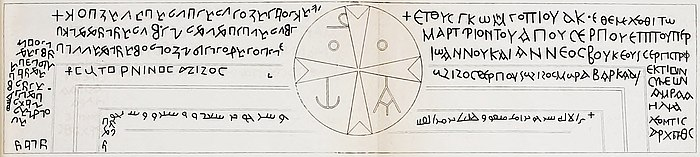
\includegraphics[width=\textwidth]{Images/image029.jpg}

autrement dit, l'écriture arabe a été utilisée par les chrétiens. Ce qui
est intéressant, c'est que l'inscription est en trois langues~: grec,
syriaque et arabe. On trouve une inscription à 100 km de Damas au roi
al-Harith datant de 538\emph{,} une inscription au sud de Damas datant
de 568, pour commémorer la construction d'un \emph{martyrum}. Qu'en
déduire~?

\begin{itemize}
\item
  On note que les premières écritures arabes sont en dehors de l'Arabie,
  ce qui plaide pour une influence syriaque dans l'émergence de l'arabe.
\item
  D'autres plaident pour une influence de l'alphabet
  nabatéen\sn{Pour rappel, les Nabatéens sont un peuple commerçant
    de l'Antiquité vivant au sud de la Jordanie et de Canaan, et au nord
    de l'actuelle Arabie. Vous avez entendu parler de Pétra~? Vous y
    êtes peut-être allés, dans ce cas vous savez déjà tout. Si vous ne
    savez pas ou si vous avez oublié, sachez que Pétra était la capitale
    de la Nabatène. Lieu magnifique. Tombé dans l'oubli, le site a été
    redécouvert en 1812 par un explorateur suisse,
    \url{http://www.hls-dhs-dss.ch/textes/f/F17075.php}{Jean-Louis
    Burckhardt} \ldots{} Une petite vidéo du ministère du tourisme
    jordanien vous donnera envie d'aller découvrir son `mystère'.
    \url{https://www.youtube.com/watch?v=YKk-JGeU_yY}{C'est ici~!}}.
\item
  En tous les cas, il semble que les premiers à parler arabe, n'étaient
  pas les Arabes. Et d'ailleurs qui sont ceux que l'on appelle Arabes~?
  Il est frappant de constater à partir des sources non musulmanes que
  ceux qui dirigent les «~conquêtes arabes~» au lendemain de la mort de
  Muḥammad ne sont pas appelés «~arabes~». On trouve les termes grecs de
  \emph{Sarakenoi} (Sarrasins), de \emph{Tayyayê'} dans les textes
  syriaques (du nom d'une tribu de l'Arabie du Nord-Est), de
  \emph{Haragènes}, de «~\emph{fils d'Ismaël}~» ou encore de
  \emph{magaritai} dans un papyrus daté de 643 ou de
  \emph{maghrâyê}\sn{Françoise \textsc{Micheau}, \emph{Les débuts
    de l'islam}, Paris, Téraèdre, 2012, p. 52.}.
\end{itemize}

La première mention du mot `arabe' se trouve sur une inscription
assyrienne~; elle date de 853 avant JC. Il y est question de la mention
d'adversaires et notamment Gindibu' l'Arabe. Plus tard, le terme
apparaît pour désigner des peuplades nomades, avec leurs chameaux.

\foreignlanguage{greek}{
Ἰουδαῖοί τε καὶ προσήλυτοι, Κρῆτες καὶ Ἄραβες, ἀκούομεν
λαλούντων αὐτῶν ταῖς ἡμετέραις γλώσσαις τὰ μεγαλεῖα τοῦ θεοῦ.} (Ac 2, la
Pentecôte)



Cela ne se limite pas à la péninsule de l'Arabie\ldots{} on désigne
aussi par Arabe ceux qui vivent au bord du Nil. On en a un bel exemple
chez Hérodote. Le terme est donc en premier lieu \textbf{employé par
l'extérieur pour désigner ces populations}. La première fois qu'elles
parlent d'elles-mêmes en se désignant par ce mot, se voit sur une
inscription du 3\textsuperscript{ème} siècle de notre ère où un individu
dit de lui qu'il est \emph{`arabī}. Il y a une inscription du
4\textsuperscript{ème} siècle, où il est question d'un groupe d'arabes.

\begin{itemize}
\item
  À la veille de l'islam, il y a donc un ensemble vaste de populations
  qui ne se désignaient pas eux-mêmes ou rarement par le terme d'arabe.
\end{itemize}

\textbf{Du coup, on se demande s'il ne s'agit pas d'une construction
\emph{a posteriori}.}

\vide{lenvironnement-religieux-de-la-puxe9ninsule-arabe}{%
\subsection{{L'environnement religieux de la
péninsule arabe
}}\label{lenvironnement-religieux-de-la-puxe9ninsule-arabe}}

Nous avons vu que La Mecque abritait un temple aux multiples divinités.
Nous avons vu aussi que des chrétiens et des juifs s'y trouvaient. Au
regard de l'histoire des royaumes voisins, il n'y a rien de surprenant.
Mais entrons un peu plus dans le détail\sn{Dans un souci
  synthétique, je m'appuie notamment sur une contribution très bien
  faite de Michel Reeber, «~Le contexte religieux de l'Arabie
  préislamique~», dans \emph{Le Coran et la Bible}, Paris, 2002, p.
  13-42.}.

\vide{le-polythuxe9isme-de-larabie-le-culte-buxe9tylique}{%
\subsubsection{{Le polythéisme de l'Arabie~: le
culte bétylique
}}\label{le-polythuxe9isme-de-larabie-le-culte-buxe9tylique}}

Si vous avez eu la curiosité de lire l'article de Jacqueline Chabbi,
vous vous souvenez probablement que les Bédouins pratiquaient le culte
des bétyles, c'est-à-dire ces roches sacrées censées être la demeure
d'un dieu (bétyle vient de \emph{bayt} -- maison et de \emph{el} -
dieu). Les pierres étaient transportées par les tribus nomades, mais à
La Mecque, cité sédentaire, on avait édifié un temple qui les abritait.
La fameuse pierre noire qui est dans l'actuelle Ka`ba n'est pas sans
rappeler cette tradition bédouine. Elle a donné lieu à de multiples
légendes. L'une d'entre elles dit qu'elle fut jetée du ciel sur terre et
que blanche elle était, mais que ce sont les péchés des hommes qui l'ont
rendue noire. Cela me rappelle une tradition chrétienne antique à propos
du baptême de Jésus~: on a pu dire que Jésus immaculé, donc de blanc
qu'il était, au moment de son baptême est ressorti noir du Jourdain car
il portait le péché des hommes\ldots{}

Il existait aussi des rituels de circumambulation autour de la Ka`ba
ainsi qu'un pèlerinage entre Marwa et Safa, le jet de pierres autour
d'une stèle, la vénération de feux sacrés. L'islam, comme nous le
verrons, garde souvent une emprunte de ces rituels, mais il les a
islamisés. En revanche, pas de feu. \textbf{Le passage au calendrier
lunaire a permis de maintenir des pratiques tout en rompant avec les
rituels solaires liés aux saisons, marquant ainsi une vraie rupture avec
les rites antéislamiques.}

Parmi les rites, on offrait aussi des sacrifices d'animaux ou même
d'êtres humains. Le Coran fait mention des sacrifices d'enfants qui
semblent être courants~:
\begin{quote}
S. 6, 137~: «~Et c'est ainsi que leurs divinités ont enjolivé à beaucoup
d'associateurs le meurtre de leurs enfants, afin de les ruiner et de
travestir à leurs yeux leur religion. Or si Allah voulait, ils ne le
feraient pas. Laisse-les donc, ainsi que ce qu'ils inventent~».
    
\end{quote}

  Ce verset pointe une pratique, mais en même temps, il est ambigu
  puisque\textbf{,} s'il montre l'horreur du massacre et ses
  conséquences funestes\textbf{,} il n'invite pas pour autant à lutter
  contre ces pratiques, comme si elles étaient voulues par Dieu et
  conduisaient \emph{in fine} à la mort des idolâtres.

Quant au Panthéon, s'il y avait plusieurs dieux, le culte de Hubal, qui
provient de Mésopotamie ou de Syrie, était prédominant\sn{Toufic
  Fahd, Le Panthéon de l'Arabie Centrale à la veille de l'Hégire,
  Institut Français d'Archéologie de Beyrouth : Bibliothèque
  archéologique et historique, n°88, 1968.}. Une statue dans le Temple
de la Ka`ba le représentait.


\paragraph{Houbal}{Divinité principale du panthéon arabe,
Houbal était connu sous le nom de « Seigneur de la Ka'ba ». Il était
probablement le père de la Triade des déesses Allât, Al-'Uzzâ et Manât,
les Filles de Houbal. En dehors de l'Arabie du sud, son nom apparaît
seulement dans une inscription nabatéenne où il est associé à deux
autres divinités, Dhu-al-Sharâ (Dusarès ; en arabe : \TArabe{ ذو الشّرى }et
Manawatu (en arabe :\TArabe{ مناة-مناواتو,} équivalent arabe nabatéen de Manât).;
'après Ibn Ishaq, la statue de la Ka'aba était une effigie
anthropomorphe en cornaline ; la Sira rapporte qu'Abd al-Muttalib ayant
promis un fils en sacrifice à Houbal qui l'avait aidé à retrouver la
source Zamzam, le sort aurait tout d'abord désigné Abdallah, père de
Mahomet. Sur les conseils d'une devineresse, on aurait proposé au dieu
cent chameaux en échange. Après dix divinations, chacune suivie d'une
augmentation du nombre des chameaux, Abdallah eut la vie sauve contre
mille chameaux.
}

\paragraph{Trois divinités} le concurrençaient. Comme nous l'avons vu, elles sont
mentionnées dans le Coran~: al-Uzzā, al-Lāt et Manāt (S. 53, 19-20).
Al-Uzzā était la déesse vénérée par les Quraysh, tribu dont est issu
Muḥammad. Selon les historiens musulmans, la Ka`ba contenait quelques
360 figurines (tiens, c'est la réponse à la question du
1\textsuperscript{er} chapitre). Muḥammad, de retour à La Mecque après
son Hégire à Médine, donnera l'assaut contre elles et les détruira
toutes, à l'exception de deux d'entre elles. \textbf{Quelles sont ces
fameuses deux icônes qu'il n'a pas fait
détruire}\sn{D'après la tradition, Mahomet, lorsqu'il investit la
  Kaaba, ordonna la destruction de toutes les idoles, sauf une : une
  icône mariale qu'il protégea de ses mains. Maryam, mère du prophète
  Jésus, Isâ (Issa), est donc vénérée partout par les musulmans.}\textbf{\ldots{}
Ce n'est pas sans incidences sur la nature des relations entre
communautés de religions différentes, ni non plus sans conséquences
aujourd'hui.} On en reparlera.

La connaissance de cette culture religieuse tribale permet d'enraciner
la compréhension de l'islam et notamment de ses rites. Mais plus encore,
elle permet de comprendre le Coran lui-même. C'est le propos de la
recherche de Jacqueline Chabbi dans son ouvrage \emph{Le Coran
décrypté}. Elle montre que certains passages s'éclairent en lien avec le
milieu tribal de Muḥammad. Ainsi, par exemple, elle remarque que bien
des métaphores eschatologiques et bibliques du Coran sont une réécriture
adaptée à la culture tribale. À cet égard, il est symptomatique que le
paradis soit décrit comme une oasis, un jardin (\emph{ğanna}) irrigué de
canaux toujours à ras bord (\emph{anḥār}), ombragés et sans soleil
(\emph{lā yarawna fihā `amsan}) (S. 76, 13)\sn{~Jacqueline Chabbi,
  «~La possibilité du Coran comme document anthropologique~», dans Mehdi
  \textsc{Azaiez} (dir.) et Sabrina \textsc{Mervin} (coll.), \emph{Le
  Coran}. Nouvelles approches, CNRS Editions, 2013, p. 189-205.}. On est
ici en plein milieu culturel arabe caractérisé par une phobie du soleil.
Ce travail sur le milieu tribal de l'Arabie antéislamique n'est pas sans
incidence dans la compréhension du Coran mais aussi dans ses
traductions. Ainsi, par exemple, la traduction de \emph{anḥār} par
fleuves, comme pour les fleuves bibliques du paradis, est un \emph{a
priori} de traduction et ne rend pas compte de sa signification exacte.
Il n'y a pas de fleuves, ni de rivières dans la péninsule arabe, juste
des points d'eau, quelques sources, parfois des lacs souterrains à
l'instar de La Mecque. De la même manière, la représentation de l'enfer
dans le Coran s'appuie sur le milieu tribal. Il est question du
\emph{ḥamīm} (S. 47, 15)~: c'est la pluie des orages d'été~; c'est lui
qui vient abreuver les damnés. Ils n'ont pour seule nourriture que le
\emph{dari'}, c'est-à-dire l'herbe à chameaux. Le \emph{nār,} traduit
par enfer, \ldots{} est en fait un feu solaire perpétuel.

Dans son dernier livre, \emph{Les trois piliers de l'islam}, elle montre
que l'islam tel qu'il se construit au cours de l'histoire est
essentiellement une construction à l'époque abbasside, époque
caractérisée par des guerres avec l'empire byzantin~; époque qui est
aussi celle d'un empire qui cherche à se démarquer de la première
dynastie des Omeyyades, époque où les textes sont fixés et notamment les
recueils de \emph{Sunna}. Or, les recenseurs ne sont pas arabes. Ils
proviennent de milieux culturels de contrées lointaines à l'Arabie~:
Buḫārī est de Transoxiane (actuel Ouzbékistan), Muslim de Nišapūr
(actuel Nors-Est de l'Iran), etc. quant à la \emph{Sunna} d'Ibn Ḥanbal,
le maître bagdadien, sa \emph{Sunna} ne fait pas partie des livres
canoniques\sn{Chabbi, Jacqueline,~\emph{Les Trois Piliers de
  l'islam}, \emph{op.cit.}, p. 15.}. Or, \textbf{leurs lectures, dans la
mesure où la Sunna est aussi l'herméneutique du Coran, vont imposer une
compréhension du Coran qui se détache du sens du Coran des origines.}
Pour l'historienne, il ne s'agit pas de rejeter ces lectures -- cela
relève de la démarche théologique, croyante -- mais de dire qu'une
attention à l'anthropologie du milieu où est prêché le Coran donne des
clefs de compréhension au texte sacré de l'islam. Pour autant, on peut
dire que Chabbi voit dans ce travail une mission salutaire~: c'est ici
que l'historienne se fait engagée~: à l'heure du fondamentalisme où des
idéologies se vantent de revenir au sens originel, il s'agit de lire le
Coran dans toute la vigueur de son verbe au-delà des lectures qui lui
furent accolées et qui lui sont encore posées.
\begin{quote}
    «~Ils lisent certes mais, ne connaissant ni les tenants ni les
aboutissants du texte, que comprennent-ils~? Texte sans contexte et sans
rattachement à un passé et à une tradition n'est que ruine du sens,
pourrait-on dire en plagiant un célèbre aphorisme~» (p.~31-32).
\end{quote}


Mais quel est ce sens originel du Coran ? Et comment le retrouver~?

L'auteur reconnaît qu'il sera difficile, voire impossible, de le
ressusciter car il prend naissance au sein d'une culture de l'oralité~;
il y a donc un «~écart sociologique~» (p.~11). Cependant, le Coran
témoigne de l'importance du milieu anthropologique, et si les références
bibliques restent parfois évasives, ce n'est pas parce qu'elles sont
connues -- ce que soutient Guillaume Dye -- mais parce qu'elles sont
réinterprétées. Or, le milieu anthropologique de l'Arabie est celui de
la culture tribale marquée par trois piliers~: \textbf{l'alliance, la
guidance et le don}. Ces piliers sont de nécessité pour les hommes de ce
milieu. Ils se retrouvent dans le Coran et doivent être abordés à partir
des sens qu'ils avaient à l'époque. Son étude lexicale lui permet aussi
d'identifier l'hétérogénéité des champs lexicaux en fonction des milieux
mecquois et médinois~: ainsi, elle remarque que le vocabulaire à Médine
y est beaucoup plus diversifié, et l'influence de l'hébreu y est plus
net. La terminologie y est aussi renouvelée. Symptomatique à cet égard
est la racine \emph{baraʾ} pour désigner la création~: si elle se trouve
au livre de la Genèse, elle est absente des versets mecquois. Plus
largement, Chabbi replace le sens du mot \emph{kitāb} -- traduit
communément par «~livre~» -- au sein de la culture de l'oralité~: il ne
s'agit pas d'un livre matériel, mais d'un message fixé oralement
(p.~58). L'univers tribal s'exprime aussi dans la nature des
descriptions eschatologiques. Ces croyances sont nouvelles et
constituent une nouveauté pour les mecquois, mais elles déploient un
code symbolique relatif au désert~qu'il s'agisse de la tempête ou du
combat contre une tribu.

Sur la nature religieuse du milieu de la péninsule arabique, elle
souligne qu'il est avant tout marqué -- et plus \textbf{à La Mecque qu'à
Médine -- par le caractère bétylique \mn{p.~117}. À cet égard, le mot
\emph{bayt} dans le Coran ne renvoie pas à un temple ou à une maison,
mais au cœur de la cité mecquoise, la Kaʿba~}: il existe une symétrie
entre la demeure de la divinité et celle des hommes puisqu'il s'agit
d'un modèle de duplication appliquée à la divinité censée les
\textbf{protéger} (p. 117).

Quant à la question des prophètes mentionnés dans le Coran, ils ont fait
l'objet d'une étude approfondie par l'islamologie\sn{~Speyer,
  Heinrich, \emph{Die Biblischen Erzählungen im Qoran,} Hildesheim, G.
  Olms, 1961 (1931).}. L'originalité de la recherche de Chabbi est de
montrer que les thèmes qui leur sont rattachés sont adaptés au monde
tribal. Ainsi, à propos de la confrontation d'Abraham avec des idoles
(\emph{asnām}), on a généralement mis en avant le rapprochement de ce
texte coranique avec le chapitre 12 du \emph{Livre des
Jubilés}\sn{Voir pour le Testament d'Abraham~: Gobillot,
  Geneviève, «~Le Coran, guide de lecture de la Bible et des textes
  apocryphes~», \emph{Pardès} 50, 2, 2011, p. 131-154.}~mais, pour
Chabbi, le cœur du message ne porte pas tant sur les pierres taillées
que sur l'opposition entre la croyance des pères (\emph{ābāʾ}) et celle
qu'il faut désormais accorder au Seigneur des peuples/tribus (\emph{Rabb
al-ʿālamīn}) (p. 97) -- non pas «~Seigneur des mondes~» selon la
traduction commune mais «~Seigneur des tribus~» --. Par conséquent, Dieu
est celui qui crée, guide, nourrit, abreuve, fait mourir et revivre. Le
Seigneur vient se substituer aux dieux incapables de protéger et de se
protéger (Cor.~26,~92-93). Dans la péninsule arabique, le \emph{Rabb},
est une figure protectrice.

 
\mn{\url{https://fr.wikipedia.org/wiki/Ar-Rahman}} 


\paragraph{Raḥmān}
L'évolution sémantique pour désigner Dieu est dans le Coran hautement
illustrative du thème de l'alliance. Ainsi, \textbf{la figure de
\emph{Raḥmān}},\TArabe{ الرحمن } \emph{le miséricordieux}~ \textbf{est propre à la
période mecquoise et disparaît au temps de Médine pour être remplacée
par celle d'\emph{Allāh}}. La notion de \emph{Rabb} renvoie à l'idée
d'un échange~; il y a une personnalisation de la relation par
l'expression \emph{Rabbī}, mon Seigneur (p. 143). Le divin est
foncièrement le \emph{walī}, c'est-à-dire le proche, le
\textbf{{protecteur}}.

Le \emph{muʾmin}\sn{(\textsc{a}.), participe actif de la
  4\textsuperscript{e}~forme de la racine~\emph{ʾmn}, signifie
  «Croyant», mais est aussi l'un des noms de Dieu (LIX, 23).}, n'est pas
d'abord celui qui croit, mais celui qui s'est rallié avec confiance.
Chabbi écrit~:
\begin{quote}
    
«~L'importance des occurrences de cette terminologie est frappante. Elle
témoigne de la spécificité de l'engagement mutuel du divin et de
l'humain, car l'alliance n'est jamais gratuite~; elle ne va pas sans
contrepartie de part et d'autre~» (p.~153).
\end{quote}
\begin{Ex}

{Quand on parle de Rahman avec un musulman, miséricorde
n'a pas forcément le même sens~: pardon pour un chrétien, bienfaisance
(pluie) pour un
musulman}
\end{Ex}

Quant au nom \emph{Rahmān}, elle remarque que si la racine hébraïque
connote l'idée de compassion et de miséricorde, sa réappropriation dans
le milieu tribal via le monde yéménite le connote de l'idée de
bienfaisance et de bienveillance. Le \emph{Rahmān} joue le rôle du Dieu
qui dispense la pluie, fonction établie à Athtar, dieu de la pluie du
Yémen (p.~127). Mais la tradition musulmane dit-elle autre chose~? Il
est frappant de constater que les traités théologiques musulmans sur les
noms divins s'inscrivent pleinement dans la définition d'une
\emph{raḥma} comprise non comme miséricorde au sens chrétien, mais
bienveillance et bienfaisance, à l'instar de celui d'al-Ġazālī \label{theol:AlGazali23}. Sur ce
point, Chabbi vient davantage corriger une traductologie influencée par
le vocabulaire théologique du christianisme que renouveler le sens
terminologique au sein de la tradition islamique.

\vide{alliance}{%
\subsubsection{Alliance}\label{alliance}}

Du point de vue du développement des idées religieuses, Chabbi souligne
l'émergence du allāhisme, mouvement de ralliement à une divinité qui
assume les fonctions assignées aux divinités d'un milieu tribal~:
alliance et protection, jugement eschatologique. Au cours de la
révélation mecquoise, \emph{Ilāh} est d'abord le dieu qui s'impose sur
les autres dieux. La notion de \emph{\textbf{walāʾ}} , ô combien
utilisée dans les milieux fondamentalistes et salafistes d'aujourd'hui,
signifie \textbf{l'alliance, la solidarité} au sein d'un même groupe
partageant le même espace.

\vide{guidance}{%
\subsubsection{Guidance}\label{guidance}}

De même, les noms divins se comprennent dans le cadre du monde tribal~:
dire de Dieu qu'il est \emph{ʿalīm}, c'est faire de lui le maître des
signes (\emph{aʿlām}) et Chabbi de préciser que cela renvoie au signe de
la piste~: \emph{Ilāh} est celui qui guide et conduit. Il connaît
l'avenir et permet de guider son groupe afin de le protéger des périls.
Ce dont il protège ce n'est pas la nuit, mais la ténèbre -- nuit sans
lune où l'on ne peut plus suivre la piste -- alors que les nuits
éclairées par la lune rendent le chemin des caravaniers aisés par
contraste avec les chaleurs de la journée. Dans le désert, la guidance
(\emph{hudā}) est de nécessité~: elle est une question de vie ou de
mort. Et si Dieu guide, c'est pour protéger de la mort non pour inviter
à en prendre le chemin. Là encore, l'analyse se fait engagée~:
\begin{quote}
«~Autant dire que les outrances actuelles qui assurent préférer la mort
dans la voie de Dieu en croyant prendre appui sur le passé premier sont
en totale contradiction avec la parole coranique telle qu'elle
s'adressait aux hommes de son temps dans la société qui était la leur~»
(p.~157).
\end{quote}

Les routes sont des chemins dangereux, surchargés d'embûches physiques
et surnaturelles, de puissances hostiles si bien que tout déplacement
est une aventure périlleuse. Dans ce contexte, les dieux préislamiques
exerçaient la fonction de guide. Les seigneurs (\emph{arbāb}) n'étaient
pas les maîtres de ces lieux mais ils pouvaient y conduire les hommes et
les guider, les protéger. Or, le sédentaire, non habitué à se déplacer,
devait pour tout déplacement recourir à des guides. \textbf{La parole
coranique exprime ce besoin~: elle n'est pas issue d'un milieu nomade,
mais sédentaire.} La thématique de la guidance permet donc à l'auteur de
restituer le sens perdu de mots clefs du vocabulaire coranique et
islamique.

\vide{ux161arux12bux2bfa-voie}{%
\paragraph{šarīʿa~, voie}\label{ux161arux12bux2bfa-voie}}

Ainsi en est-il de \emph{šarīʿa}~: elle est la voie donnée pour éviter
de se perdre~: elle est grâce accordée à Muḥammad alors que les enfants
d'Israël se sont écartés du chemin, bien que Dieu les avait favorisés
(\emph{tafdīl}) (Cor.~45,~15-18). Cette voie renvoie à un point d'eau où
l'eau affleure, ce qui permet aux dromadaires de s'y désaltérer sans que
l'on doive aller y puiser~: c'est donc un lieu facile d'accès. Ainsi,
Dieu, par la \emph{šarīʿa}~donne accès à l'eau~; il dispose de
ressources qu'il partage. Par suite, perdre la voie conduit au malheur,
à l'exemple des fils d'Israël (Cor.~45, 17). En conclusion, Chabbi
remarque que le Coran est loin de la signification qui sera donnée à ce
terme et qui ne date que du iii\textsuperscript{e} siècle de l'Hégire
(p.~177). Elle conclut aussi que l'intégration de châtiments corporels à
la \emph{šarīʿa}~est impossible en milieu pré-islamique et se trouve aux
antipodes des solidarités qui s'y nouaient. La seule disposition légale
qui se retrouve dans le Coran est celle du \emph{qiṣāṣ}, le prix du sang
(Cor.~4, 92).

\vide{lapidation-mentionnuxe9e-dans-la-sira}{%
\subsubsection{Lapidation mentionnée dans la
sira~?}\label{lapidation-mentionnuxe9e-dans-la-sira}}

Quant à la lapidation (\emph{raǧm}), elle était pratiquée non pour tuer,
mais pour éloigner l'indésirable à l'exemple des puissances maléfiques
dont il s'agit de se prémunir pour éviter de subir leur malfaisance (p.
178) (Cor. 86, 25~; Cor. 15, 17, 34).

\vide{la-sunna-la-piste-sure}{%
\paragraph{La sunna, la piste sure}\label{la-sunna-la-piste-sure}}

De même, si le mot \emph{Sunna} désigne la piste sûre, réputée,
attribuée à Dieu, la \emph{Sunna d'Allāh} est une voie de châtiment pour
ceux qui ont trahi l'alliance. Elle n'est pas un modèle à suivre, sens
qui sera donné à propos de Muḥammad. Cette expression, typique du
sunnisme, a cherché à se fonder sur le Coran à partir du mot
\emph{uswa}, se rallier à\emph{.} Ainsi, Abraham a-t-il été présenté
comme un exemple à suivre en tant qu'il a rompu avec l'allégeance des
dieux de ses pères (Cor. 60, 4 et 6). De même, le messager d'Allāh
(désigné comme Muḥammad par les commentateurs) est-il présenté comme un
exemple à suivre (S.~33, 21). Mais pour Chabbi, le contexte n'est pas
celui du modèle, mais de l'alliance~: il est celui qui s'est rallié à
Dieu. La \textbf{Sunna de Dieu renvoie donc à une coutume divine~qui
consiste à rejeter, à faire disparaître celui qui s'éloigne ou qui
accuse le messager de Dieu de mensonge.}

À propos du terme \emph{umma}, communément traduit par «~communauté~»,
Chabbi souligne que dans le Coran, là aussi, il désigne la bonne voie :
«~Nous avons trouvé nos pères sur une \emph{umma} et c'est assurément
leurs traces qui nous sont modèle {[}pour suivre la route{]} \emph{ʿalā
aṯāri-him muqtadūn}~» (Cor. 43, 22). Quant au \emph{ǧihād}, si on a
souligné à maintes reprises qu'il est un effort, Chabbi resitue cet
effort par rapport au milieu local où le sédentaire est désigné comme
celui qui reste sur place (p. 194). Dans un monde où la chaleur brûle
les corps, tout déplacement est un enfer. Face à la tentation de
s'installer, le Coran affirme que le paradis leur sera interdit.
\textbf{Aussi, l'image du paradis renvoie-t-elle à un monde immobile,
sans activité.} Il est la récompense accordée à la suite de à l'effort
engagé dans les pas de Muḥammad. D'où les images eschatologiques comme
celles de l'accoudement (\emph{ittikāʾ}). «~Le paradis coranique semble
ainsi avoir horreur du mouvement. Il fige les élus dans l'immobilité
d'un repos qui les fait en quelque sorte échapper à la course harassante
pour la vie qui avait été leur lot durant leur vie~» (p. 293).

\vide{ux1e7ihux101d-combat-pour-la-voie-dallux101h-dans-un-monde-ouxf9-le-paradis-est-limmobilituxe9}{%
\paragraph{Ǧihād, combat pour la voie d'Allāh dans un monde où le
paradis est
l'immobilité}\label{ux1e7ihux101d-combat-pour-la-voie-dallux101h-dans-un-monde-ouxf9-le-paradis-est-limmobilituxe9}}

Le \emph{ǧihād} devient le combat à mener dans la voie d'Allāh, il est
le \emph{qitāl}. Et traduire \emph{qitāl} par le fait de tuer est une
altération de sens car il ne s'agit pas de tuer pour tuer, mais il
s'agit de combattre en sachant que ce combat peut conduire à la mort (p.
200-201). Mais «~tuer les hommes d'un groupe adverse de manière
inconsidérée ou gratuitement massacreuse constitue une transgression
majeure~» (p. 203).


\mn{Combien est vil le prix contre lequel ils ont troqué
leurs âmes lorsqu'ils ont nié ce que Dieu a révélé et ce, uniquement par
dépit, car ils n'ont pu admettre que Dieu, par un effet de Sa grâce, ait
choisi certains de Ses serviteurs pour les gratifier de la révélation !
Ils se sont ainsi attirés doublement la colère du Seigneur et le
châtiment ignominieux qui sera réservé aux
infidèles.}



Le verset Cor. 2, 90 rappelle à cet égard qu'il ne faut pas commettre
d'agression (inconsidérée), que Dieu n'aime pas les agresseurs
(\emph{muʿtadīn}).

Par opposition, la négociation qui permet de répondre au risque encouru
est considérée comme un don (\emph{fatḥ}). Le chapitre consacré à la
violence permet ainsi de rappeler que dans tous les cas, l'action de la
violence revient à la divinité. L'exacerbation de la parole coranique
doit être lue comme la conséquence de l'immobilisme des hommes. À
Médine, le prophète réclame l'obéissance (\emph{tāʿa})~; il y a ici une
rupture avec La Mecque où le Coran orientait sur l'obéissance à la
divinité.

\begin{table}[h!]
    \centering
    \small
   \begin{tabular}{p{0.45\textwidth}p{0.45\textwidth} }
À l'expiration des mois sacrés, tuez les polythéistes partout où vous
les trouverez ! Capturez-les ! Assiégez-les ! Dressez-leur des
embuscades ! S'ils se repentent, s'ils accomplissent la salât, s'ils
s'acquittent de la zakât, laissez-les en paix, car Dieu est Clément et
Miséricordieux. & Faitha insalakha alashhuru alhurumu faoqtuloo
almushrikeena haythu wajadtumoohum wakhuthoohum waohsuroohum waoqAAudoo
lahum kulla marsadin fain taboo waaqamoo alssalata waatawoo alzzakata
fakhalloo sabeelahum inna Allaha ghafoorun raheemun (⁎) \\
 
\end{tabular}
\sidecaption{verset dit du sabre (Cor. 9, 5)}
\end{table}

À propos du verset dit du sabre (Cor. 9, 5), la précision temporelle
«~après les mois sacrés~», montre une mise en conformité avec les règles
tribales (p.~249). L'injonction «~tuez-les~» est incompatible avec le
contexte du verset qui invite à accueillir les repentants~: il s'agit
donc d'abord de combattre~; par ailleurs cet appel est une réponse à une
agression antérieure.

\vide{don}{%
\subsubsection{Don}\label{don}}

Enfin, concernant le don, il est mutuel (p.~265). Conformément à ce
qu'avait montré Mauss, celui qui ne peut donner est dans une situation
très faible car \textbf{le don est aussi une marque de pouvoir}. Par
conséquent, \textbf{l'orphelin} a la position la plus inférieure. Dans
la logique du don coranique, il s'agit de donner, mais sans s'appauvrir
soi-même. Pour autant, le don appelle le contre don et Chabbi propose
une interprétation très intéressante du \emph{\textbf{kufr}} traduit
habituellement par \textbf{infidélité} ou mécréance. Pour elle, il
désigne \textbf{l'ingratitude}~: «~ce serait un moyen de se soustraire à
une obligation sociale en masquant la bienfaisance dont on a été
bénéficiaire~» (p.~266). La thématique du don divin est typiquement
tribale. Les délices du paradis, le repos eschatologique, sont la
récompense de la divinité à celui qui se sera investi dans ce monde et
aura su répondre à ses obligations. Mais le don n'est pas seulement lié
au futur. Dès ici-bas, la divinité offre~: ce sont les dons de
subsistance. Dieu est celui qui offre ces pâturages verdoyants, et parmi
les traductions originales avancées dans l'ouvrage, pour Chabbi,
traduire le verset Cor. 16, 80 par «~peut-être deviendrez-vous
musulmans~» est un anachronisme~: dans le contexte tribal, il s'agit
d'accepter de se mettre sous la garde de la divinité qui assure ces
bienfaits. Chabbi propose~: «~peut-être accepterez-vous de vous mettre
sous sa garde {[}dans la mesure où son alliance vous apporte tant
d'avantage en natures{]}~» (p. 330).

\vide{le-judauxefsme-dans-larabie-pruxe9islamique}{%
\paragraph{1.2.2 Le judaïsme dans l'Arabie
préislamique}\label{le-judauxefsme-dans-larabie-pruxe9islamique}}

À la suite de la destruction du Temple en 70, d'importantes communautés
juives émigrèrent au Moyen-Orient, en Babylonie, en Égypte, en Afrique
du Nord, à Byzance, en Italie. Certains juifs ont aussi émigré dans le
Hijāz (Arabie). La Mishna (compilation des enseignements de la loi
juive) rédigée en 200-220, en fait mention. On a pu identifier la
présence d'une vingtaine de tribus juives.

Il existait aussi une importante communauté juive dans le sud de la
péninsule arabique (Yémen). Les rois de Himyar ont fait le choix de
rejeter le polythéisme et après 380 on ne trouve plus dans tout le Yémen
la moindre inscription explicitement païenne. Cette rupture est très
profonde et se voit dans le vocabulaire avec l'usage d'une terminologie
araméenne et hébraïque comme \emph{amen}, `\emph{ālam} (monde),
\emph{bâraka} (bénir), \emph{shalôm}, \emph{salāt} (prière),
\emph{zakât} (grâce). Au début du VIème siècle, le judaïsme est la
religion dominante dans le royaume de Himyar\sn{Iwona Gajda, Le
  royaume de Himyar à l'époque monothéiste -- L'histoire de l'Arabie du
  Sud ancienne de la fin du IVe siècle de l'ère chrétienne jusqu'à
  l'avènement de l'islam.}. Avec l'unification de l'Arabie méridionale,
au 3\textsuperscript{ème} siècle, les rois de Himyar interviennent dans
l'Arabie désertique.

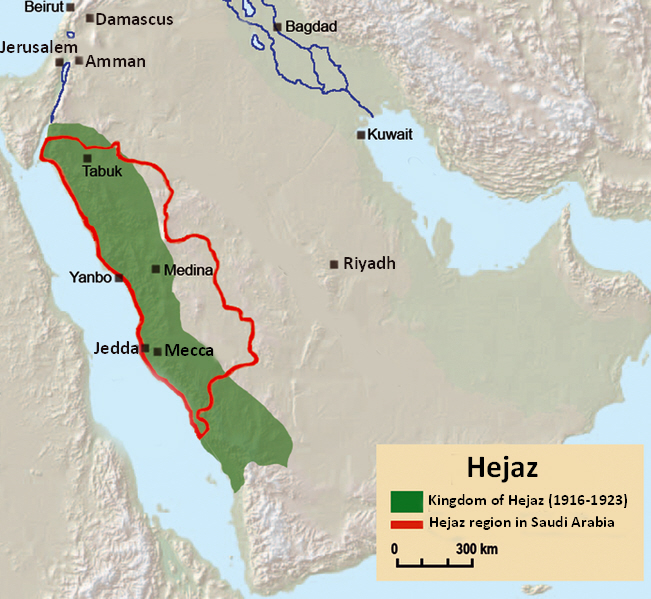
\includegraphics[width=\textwidth]{Images/image030.jpg}

Si globalement les juifs \mn{pour plus de détail sur le rapport entre Islam et judaisme, voir \cite{BarAsher:JuifsCoran}} refusèrent de se convertir à l'islam,
l'historiographie musulmane retient la conversion de certains d'entre
eux. Le plus connu est `Abd Allāh Ibn Salām, docteur de la Loi juive. Il
contribua à prêcher la conformité de la venue de Muḥammad avec la Torah.
Il est important de voir que ces premiers convertis apportent avec eux
leur culture biblique. Cela leur sera d'ailleurs reproché, comme ce fut
le cas pour un autre rabbin, Ka'b al-Akhbār. Retenez bien ce point quand
on parlera du Coran et de sa rhétorique~\ldots{} qui est très sémite.
Mais ces juifs qui fréquentent Muḥammad ou qui se convertissent dans les
premières décennies de l'islam, qui sont-ils exactement~? À quel courant
du judaïsme les rattacher~? De ce que le Coran rapporte concernant leurs
croyances sur Dieu, les anges, la création, la loi, le péché,
l'eschatologie, il semble que l'on puisse voir un lien de filiation avec
le judaïsme talmudique. Certains y ont vu des hétérodoxes juifs, mais
l'orientaliste Geiger\sn{A. \textsc{Geiger}, \emph{Was hat
  Mohammed aus dem Judenthum aufgenommen}, Bonn, 1833.}, à la lumière du
caractère sommaire des croyances juives telles qu'elles sont rapportées
par Muḥammad, suggère plutôt que les informateurs juifs de Muḥammad
étaient ignorants de leurs propres traditions -- autrement dit, il nous
invite à ne pas réduire le judaïsme de l'époque à ce que les
informateurs ont dû en rapporter. Cela rappelle un prisme méthodologique
dénoncé par al-Ġazālī \label{theol:AlGazali24} dans le \emph{Munqiḏ min al-ḍalāl} et que nous
avons vu dans la leçon précédente. Si vous avez oublié, relisez~:
\textbf{al-Ġazālī vérifie ce qu'il a compris d'une croyance auprès
d'autres membres de cette croyance.}

À La Mecque (lieu où commence la prédication de Muḥammad en 610), il est
difficile d'évaluer l'importance de la communauté juive. Mais les
versets coraniques révélés dans cette première période témoignent de
relations positives et fructueuses. La direction de la prière est
Jérusalem, le jour du jeûne (\emph{`ashūrā'}) rappelle le Yôm Kippour,
et le Coran reconnaît l'élection des juifs.
\begin{quote}
    «~Ô enfants d'Israël, souvenez-vous des bienfaits dont je vous ai
comblés~: souvenez-vous que je vous ai élevés au-dessus de tous les
humains~» (S. 2, 46).
\end{quote}


Mais à Yathrib (Médine), les juifs étaient plus nombreux.

Médine est située à 350 km de La Mecque. C'est une oasis. Il y avait une
école où l'on apprenait l'hébreu. Un des secrétaires de Muḥammad qui
sera chargé de collecter les sourates, Zayd Ibn Thābit, aurait fréquenté
cette école. En 622, au moment où Muḥammad doit fuir La Mecque et où il
va s'installer à Médine, il y a trois grandes tribus juives~: les Banū
Qurayẓa, les Banū al-Nadhîr et les Banū Qaynukā'. Ils avaient en leur
possession des terres riches et détenaient le pouvoir local. Peu à peu,
leur puissance déclina avec l'arrivée de deux tribus arabes, les Aws et
les Khazraj.

Il semble que les relations entre Muḥammad et les juifs de Médine furent
bonnes à son arrivée. Un document, «~La charte de Médine~» semble aller
dans ce sens.

\vide{clauses-en-rapport-avec-les-musulmans-et-les-croyants-monothuxe9istes}{%
\subsubsection{Clauses en rapport avec les musulmans et les croyants
monothéistes}\label{clauses-en-rapport-avec-les-musulmans-et-les-croyants-monothuxe9istes}}
\begin{quote}
 
 
 
{Les émigrés Qoraïchites et de Yathrib (Médine) et ceux
qui les suivirent et luttèrent avec eux forment une seule communauté à
part. Tous les musulmans quelles que soient leurs tribus ou
clans partagent entre eux le prix du sang, payent la rançon des captifs
selon le bon usage et
l'équité.
Les croyants monothéistes ne délaissent jamais un endetté
qui a la charge d'une famille ; ils lui donnent des fonds destiné à
payer le prix du sang ou le rachat d'un
captif.Tous les croyants monothéistes devront s'unir contre
quiconque étant rebelle ou cherchant à promouvoir l'hostilité ou la
sédition, quels que soient leurs liens familiaux ou
tribaux.  Aucun croyant monothéiste ne doit en tuer un autre, ou
soutenir un non croyant au détriment d'un
croyant.La protection de Dieu est sur tous les croyants
monothéistes, indépendamment de leur classe ou de leur origine
tribale.} 
 
 
{Il est défendu à un croyant monothéiste ayant consenti à
ce qui est écrit dans ce texte et cru en Dieu et au jour du jugement de
secourir un criminel ou de l'héberger. S'il le fait, il sera maudit par
Dieu au jour de la résurrection, sans pitié, et l'on n'acceptera de lui
ni compensation, ni
indemnité.}
 \end{quote}
     
\paragraph{{Clauses en rapport avec les
juifs.}} 
 \begin{quote}
Les juifs ne font qu'une communauté avec les
croyants. Les juifs peuvent continuer de professer leur religion et
la liberté de pratiquer leur religion est
garantie.   Tout juif qui adhère à cette charte doit avoir l'aide et
l'assistance des croyants et tous les droits des croyants doivent lui
être
donnés.Chaque tribu et chaque clan juif est responsable de son
prix du sang, de ses taxes de châtiment et de ses payements de
rançon.
  \end{quote} 
\paragraph{Clauses communes à
tous.} 
 \begin{quote}
Les juifs et les croyants monothéistes de Médine ont un
pacte de défense mutuelle entre deux groupes. Pour honorer ce pacte, ils
doivent en payer le coût
nécessaire. Les juifs et les croyants monothéistes de Médine se
conseilleront et leurs relations mutuelles doivent être fondées sur la
droiture, alors que le péché est
interdit. Aucun des juifs ou des croyants monothéistes ne doit
commettre de péchés portant préjudice à l'autre
groupe. Si les juifs font du tort aux croyants monothéistes ou si
ceux-ci font du tort à ceux-là, alors le parti lésé doit être
aidé. Médine doit rester un lieu sacré et inviolé pour tous
ceux qui joignent la charte, à l'exception de ceux qui ont commis une
injustice ou un
crime. Tous les participants à cette charte doivent boycotter
les Koraïchites non-musulmans de La
Mecque. Tous les participants à cette charte doivent défendre
Médine de toute attaque
étrangère. Aucune clause de cette charte ne doit interdire à aucun
parti de demander un châtiment
légal. Aucun participant à cette charte ne peut déclarer une
guerre sans la permission du prophète de l'islam
Mahomet. Chaque fois qu'un désaccord s'élève entre deux
participants à cette charte, le désaccord doit être soumis à Dieu et à
son messager pour
arbitrage.

 

    
\end{quote}
Document dont l'authenticité est admise. Document très important que
l'on trouvera en annexe. Mais celles-ci se détériorèrent peu à peu,
sans-doute parce que les juifs refusèrent de suivre Muḥammad dans sa
prédication de l'islam. Lorsque la rupture est consommée, la thématique
coranique change. L'islam ne s'inscrit plus dans la continuité du
judaïsme mais comme une restauration de la religion primitive,
pré-israélite, et falsifiée par les juifs.

Ici une remarque épistémologique s'impose. Les versets coraniques dans
leur diversité de ton sont lus à la lumière de l'évolution des relations
entre Muḥammad et les juifs. Mais dans quelle mesure cette histoire n'a
pas été écrite \emph{a posteriori}~? Autrement dit, n'a-t-on pas établi
une chronologie des versets -- celui-ci est de La Mecque, celui-là de
Médine -- sur la base d'un récit narratif historique qui est une
construction~? D'où la question, ce récit est-il authentique~?
D'ailleurs, la dégradation des relations avec les Juifs à Médine colle
assez mal avec la Charte de Médine.

C'est en tous les cas à cette période, que le sens de la direction de la
prière serait devenu La Mecque, et c'est à cette période que l'on
rattache les versets coraniques les plus hostiles aux juifs~:

\begin{quote}
    

«~Tu connaîtras que ceux qui nourrissent la haine la plus virulente
contre les croyants sont les juifs et les idolâtres et que ceux qui sont
les plus disposés à les aimer sont les hommes qui se disent chrétiens~»
(S. 5, 82).

«~Ceux qui ont reçu le Pentateuque, et qui ne l'observent pas,
ressemblent à l'âne qui porte des livres. C'est à quelque chose de vil
que ressemblent les hommes qui traitent les signes de Dieu de mensonges.
Dieu ne guidera point les impies~» (S. 62, 5).
\end{quote}
Dans ce contexte, Muḥammad trouve dans les deux tribus arabes des alliés
et très vite, les tribus juives sont considérées comme des ennemis. Les
juifs sont accusés d'avoir pactisé avec les gens de La Mecque, d'avoir
trahi le contrat établi avec les musulmans dans le cadre de la Charte de
Médine. Il s'ensuit un conflit violent. La guerre est d'abord déclarée
avec la tribu des Qaynuqā` qui doit fuir vers la Palestine. La
\emph{Sīra} raconte les batailles contre les juifs, ainsi que de
nombreux massacres. Vous souvenez-vous que nous avons déjà rencontré le
mot \emph{Sīra}~? Vous souvenez-vous de sa signification~?

\begin{marginfigure}
    \centering
    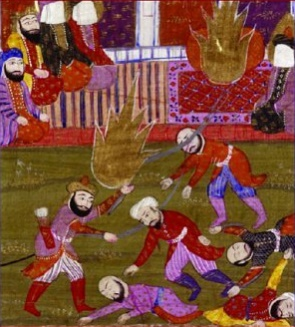
\includegraphics[width=1.31707in,height=1.45946in]{Images/image031.jpg}
    \caption{miniature du
19\textsuperscript{ème} siècle où l'on voit `Alī et Muḥammad massacrer
les membres de la tribu des Banū Qurayẓa. Manuscrit (17 folio 108b),
British Library.}
   
\end{marginfigure}
 
 



\paragraph{Le christianisme en
Arabie}

Un des archéologues, spécialiste du christianisme de la péninsule arabe,
est Christian Robin. {Le 18.08.2013, Sébastien de Courtois, dans l'émission
«~foi et tradition~» de France Culture, l'interroge. Il lui demande~tout
de go~: «~Alors Monsieur Robin, il y a eu une présence chrétienne en
Arabie
saoudite~?~»} 

Le Yémen a donc été «~officiellement~» chrétien entre 530 et 570. Son
roi est Abraha et, comme le dit Robin, on a découvert une inscription
qui date de 552 où sont mentionnées les régions soumises à son pouvoir~:
Arabie orientale, Arabie du Nord, Arabie du Nord-Est~; il y est aussi
question de Yathrib. Abraha a fait construire une cathédrale à San`ā'
{[}on est ici dans le sud de l'Arabie, l'Arabie heureuse{]} qui devient
capitale du Yémen, en 550. \emph{Les Chroniques} en donnent une
description détaillée, sublime. La cathédrale sera détruite au
8\textsuperscript{e} siècle.

Parmi les inscriptions, on dispose aussi d'une invocation à la Trinité
(\emph{Rahmanan}, son Fils \emph{Christos}, et l'Esprit Saint). Ce roi a
donc christianisé le Yémen et on ne trouve plus sous son règne
d'inscriptions spécifiquement juives.

\begin{marginfigure}
    \centering
    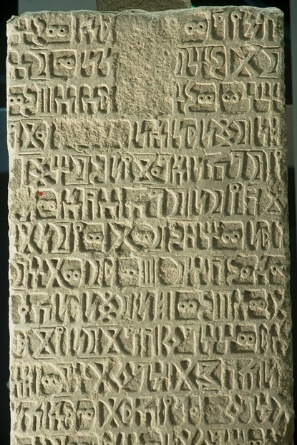
\includegraphics[width=1.31747in,height=1.96757in]{Images/image033.jpg}
    \caption{Inscription d'Abraha, 
    roi Éthiopien du Yémen, commémorant une réparation de la Digue de Marib }

\end{marginfigure}


le roi
Éthiopien du Yémen lors de la commémoration de la réparation de la Digue
de Marib et la consécration d'une église.~On y trouve aux premiers mots
l'invocation~
\begin{quote}
    « Avec la puissance, l'aide et la miséricorde de Rahmânân,
de son Messie et de l'Esprit Saint~» 
Christian Robin
\end{quote}

Mais la présence chrétienne dans le Yémen date déjà du
5\textsuperscript{e} siècle~: dans la \emph{Chronique de
Séert}\sn{Il s'agit d'une Chronique nestorienne d'auteur anonyme.
  Originellement écrite en syriaque, elle a été traduite en arabe.}, il
est question d'un commerçant de Najrān qui se serait converti lors d'un
séjour à al-Ḥīra en Irak.

Après quelques années, le chef de l'armée éthiopienne renverse le roi
installé et prend sa place. On a donc \textbf{un roi éthiopien sur le
trône du Yémen}, \textbf{en rupture avec l'Éthiopie}, qui affirme une
foi chrétienne, mais différente de son prédécesseur~: \textbf{son
lexique vient du syriaque et non de l'éthiopien}. Par ailleurs, il
supprime l'expression fils et parle de son messie. \textbf{Cela
ressemble à la christologie du Coran~: le Messie n'est plus appelé et
reconnu comme fils de Dieu.}

Dans le reste de la péninsule, il y a bien sûr une présence du
christianisme dans l'extrême nord-ouest. Byzance y joue un rôle
d'autorité. On trouve des communautés et des monastères sur la côte du
Golfe arabo-persique comme en témoignent des vestiges de ruines de
couvents découverts au Koweït, en Arabie saoudite et aux Émirats arabes
unis.

On trouve au Yémen une inscription monothéiste datant de 320~: c'est une
rupture avec les inscriptions païennes, mais également des inscriptions,
toujours du 4\textsuperscript{ème} siècle, utilisant un lexique nouveau,
emprunté au judéo-araméen. On y invoque un Dieu unique, souvent appelé
le Seigneur du ciel et de la terre. Probablement, le judaïsme a
influencé ces inscriptions.

\vide{luxe9sotuxe9risme-et-la-gnose-de-perse}{%
\paragraph{{1.2.4 L'ésotérisme et la gnose de Perse
}{1.2.4 L'ésotérisme et la gnose de Perse }}\label{luxe9sotuxe9risme-et-la-gnose-de-perse}}

Parmi les courants religieux présents en Arabie, il faut aussi faire
mention du mazdéisme et du manichéisme\sn{~Guy Monnot,
  \emph{Penseurs musulmans et religions iraniennes}, Études musulmanes
  n°16, Paris, Vrin, 1974.}. Tous deux ont joué un rôle non négligeable
dans la naissance de l'islam.

Le Coran évoque les mages (S. 22, 17), membres des castes mazdéennes.


\begin{quote}
{22. 17 }
{Certes, ceux qui croient, ceux qui pratiquent le judaïsme
ainsi que les sabéens, les chrétiens, les zoroastriens et les
polythéistes, Dieu les départagera le Jour de la Résurrection, car Il
est Témoin de toute
chose.}
{Inna allatheena amanoo waallatheena hadoo
waalssabieena waalnnasara waalmajoosa waallatheena ashrakoo inna Allaha
yafsilu baynahum yawma alqiyamati inna Allaha AAala kulli shayin
shaheedun
}
\end{quote}
\begin{marginfigure}
    \centering
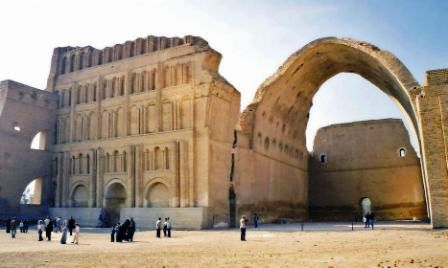
\includegraphics[width=\textwidth]{Images/image034.jpg}
    \caption{Tāq de Ctésiphon (Madā'in) en
Irak, à proximité duquel est enterré Salmān le
Perse}
    \label{fig:Ctesiphon}
\end{marginfigure}
Le mazdéisme est la religion officielle des Sassanides, dynastie perse
de 226 à 651. Mais on trouve des mazdéens en Irak, à Bahrayn, à Oman. Il
était pratiqué à La Mecque et Médine et au Yémen. Si les mazdéens
pratiquaient le rite du feu -- qui ne se retrouve pas en islam -- on
retrouve aussi dans leur religion \textbf{les cinq prières quotidiennes,
les rituels de prosternation, les rites d'ablution, la récitation de
textes sacrés, les sacrifices d'animaux}. Avant chaque geste important,
on prononçait la formule «~Au nom de Dieu~» qui trouve son pendant en
islam avec la \emph{basmala} que l'on récite avant les usages cultuels.
Au sein du mazdéisme, on trouve l'idée qu'il ne suffit pas de pratiquer,
mais que la pratique doit être motivée par l'intention. En islam, c'est
la \emph{niya} qui doit être formulée au début de chaque prière
quotidienne. \textbf{Sur le plan de la foi, le mazdéisme affirme
l'existence d'un créateur universel, d'une divinité dotée des attributs
de miséricorde, de justice, de bonté, il développe une vision
anthropologique où l'homme est d'abord parfait}~; du point de vue
eschatologique, il soutient la rétribution selon les actes posés et
l'épreuve de la pesée. Après la mort, l'âme reste auprès du mort avant
d'entreprendre un voyage. Là, elle passe sur le pont de Cinvad ~: pour
le juste, le pont s'élargit et conduit au paradis, mais pour le méchant,
il se rétrécit, devient fin comme une lame de rasoir, si bien qu'il
tombe dans les affres de l'enfer \textbf{Or, tous ces éléments se
retrouvent en islam}. Parmi les compagnons de Muḥammad, on compte un
mazdéen Salmān al-Fārisī (~m. 656), dit aussi Salmān le Perse, d'abord
converti au christianisme puis à l'islam et qui est considéré par Louis
Massignon, comme l'initiateur de l'islam iranien. Pour Louis Massignon
(nous avons déjà parlé de l'importance qu'il joua dans l'orientalisme du
vingtième siècle~et dit qu'il imposa l'usage du mot islam sur celui
d'islamisme, pour désigner la religion des musulmans), Salmān n'aurait
pas renié le Christ et serait donc un de ces personnages faisant la
jonction entre le christianisme et l'islam. Il a une grande importance
pour Massignon, car c'est près de sa tombe, un soir de mai 1908, que
celui-ci éprouva la «~Visitation de l'étranger~», qui comme un feu divin
est venu raviver les braises de sa foi\sn{Louis Massignon,
  «~Salmân ou les prémices spirituelles de l'Islam iranien~», in
  \emph{Parole donnée}, 1934.}.
\FloatBarrier



Pour ce qui est du \textbf{manichéisme}, il est apparu comme un courant
hétérodoxe du zoroastrisme, s'inspirant à la fois du bouddhisme, du
christianisme, du judaïsme, de la gnose, sur le fond du mazdéisme. C'est
une religion à vocation universelle, missionnaire donc, qui a pénétré la
péninsule arabique. Le père du premier calife omeyyade, Mu'āwiya, était
manichéen. Un certain nombre de particularités se retrouvent en islam.
Ainsi, par exemple, le \textbf{grand jeûne annuel des manichéens de
trente jours n'est pas sans rappeler le jeûne du Ramadan} -- durée
inconnue dans la Bible -- ou encore, l'interprétation de la tradition
musulmane selon laquelle Christ aurait été remplacé sur la croix par un
sosie (interprétation qui découle du commentaire du verset 4, 157~: les
juifs disent nous avons tué le Christ, mais ils ne l'ont ni tué, ni
crucifié, mais son sosie a été substitué à leurs yeux (\emph{šubbiha
la-hum}). Mais la ressemblance entre manichéisme et islam la plus
marquante concerne la prophétologie. \textbf{Le manichéisme est une
religion du Livre. Mani a reçu la visite de l'Ange de la prophétie et a
consigné dans un livre les révélations}. Contrairement à Zoroastre,
Jésus ou Bouddha, qui n'ont pas écrit eux-mêmes, la nouveauté consiste
en la rédaction personnelle du livre, évitant les falsifications opérées
par les disciples. Ce thème de la falsification des écritures se
retrouvera en islam. Notons aussi l'expression «~sceau des prophètes~».
Mani la fait sienne. Muḥammad sera ainsi appelé dans le Coran (S. 33,
40)
\begin{quote}
Muḥammad n'a jamais été le père d'un seul de vos hommes mais le messager
de Dieu, le \textbf{sceau des prophètes}, et Allāh est savant en toutes
choses.

\textbf{\TArabe{مَا كَانَ مُحَمَّدٌ أَبَا أَحَدٍ مِنْ رِجَالِكُمْ وَلَكِنْ
رَسُولَ اللَّهِ وَخَاتَمَ النَّبِيِّينَ وَكَانَ اللَّهُ بِكُلِّ شَيْءٍ
عَلِيمًا}}
\end{quote}


\section{Repères chronologiques et histoire des premiers
califes}

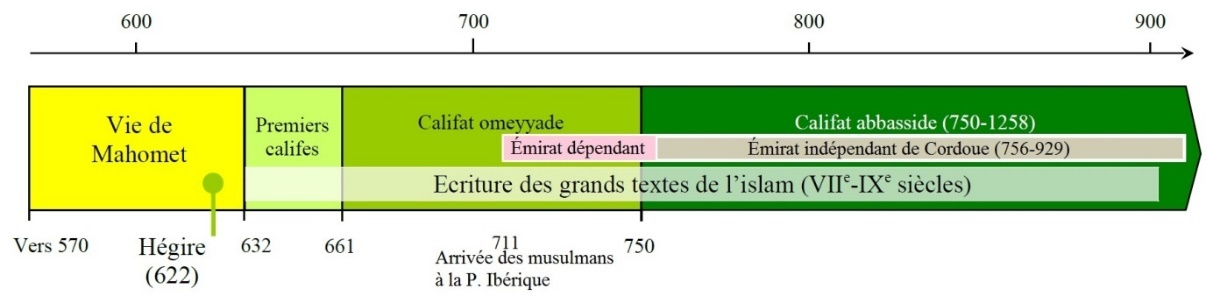
\includegraphics[width=\textwidth]{Images/image035.jpg}

Selon la tradition musulmane, Muḥammad est né vers 570. C'est en 610
qu'a lieu la première manifestation de la révélation du Coran -- nous y
reviendrons. 622 est l'année de l'hégire (\emph{hiǧra} en arabe)~: elle
renvoie au départ de Muḥammad de La Mecque pour Médine. Traduit parfois
par émigration, fuite (la vie de Muḥammad et des siens est menacée par
les Mecquois), la racine souligne l'idée de rupture des liens amicaux ou
familiaux.

\begin{Def}[muhāǧirūn et anṣār]
On appelle les Mecquois qui partirent avec Muḥammad
\textbf{les \emph{muhāǧirūn}, les émigrés.} Les Médinois qui se
convertirent à l'islam sont appelés \textbf{les \emph{anṣār}, les
auxiliaires}.
\end{Def}
La racine NaṢaRa signifiant venir en aide, apporter
protection.
Au moment du choix des premiers califes, grande sera la rivalité entre
les \emph{muhāǧirūn} et les \emph{anṣārs} où les appartenances tribales
ressurgissent.

La \emph{hiǧra} est au cœur du projet islamiste de Daesh qui a appelé
tous les musulmans à le rejoindre et à ainsi mettre ses pas dans ceux de
Muḥammad et de son émigration.

Les premiers califes sont désignés \emph{al-rāšidūn}, c'est-à-dire les
Bien-Guidés. C'est la période des quatre premiers califes~; dans l'ordre
chronologique~: Abū Bakr, ʿUmar, ʿUṯmān et ʿAlī.

\vide{abux16b-bakr-m.-634}{%
\subsubsection{{Abū Bakr (m. 634)
}{Abū Bakr (m. 634) }}\label{abux16b-bakr-m.-634}}

La tradition sunnite fait de lui le premier musulman après Ḫadiǧa,
l'épouse du jeune Muḥammad. Cette tradition permet aussi de légitimer le
rôle d'Abū Bakr et son institution comme calife, à l'issue de la mort de
Muḥammad, dans un contexte fébrile. D'ailleurs, sur la question de
savoir qui est le premier à avoir endossé l'islam, les šīʿites
considèrent quant à eux que c'est ʿAlī. À la mort de Muḥammad, une
élection eut lieu dans un contexte tendu où les opposants à Abū Bakr
furent absents et ne purent donc se prononcer. Par suite, un grand
mouvement se souleva pour s'opposer à ce choix. Certains refusèrent de
payer la zakāt. On appelle ce temps la période de la grande apostasie
(\emph{ridda}). Mais il faut bien voir qu'il s'agissait plus de
contester l'autorité d'Abū Bakr que de rejeter l'islam. Mais Abū Bakr et
ses partisans virent dans le non-paiement de la \emph{zakāt}, laquelle
est un pilier de l'islam, un acte d'apostasie. Il partit en guerre
contre les tribus récalcitrantes. La bataille d'al-Yamāma vit la mort de
plus de 1200 musulmans et 39 compagnons. Il meurt de maladie.

\vide{ux2bfumar-m.-644}{%
\subsubsection{ʿUmar (m. 644)}\label{ux2bfumar-m.-644}}

Il appartient à la tribu des Qurayš. Il a été nommé par Abū Bakr pour
lui succéder, après que ce dernier a consulté les compagnons. On le
surnomme \emph{al-Fārūq}, l'Équitable. Il fut l'un des premiers
opposants à l'islam et un défenseur des traditions mecquoises. Dans
certains récits sunnites, il est présenté comme ayant torturé des
musulmans pour qu'ils renient leur foi à l'exemple d'une servante des
Banū Mūʾammil. L'hégire dont nous avons parlé fut décidé par Muḥammad
dans le contexte de ces persécutions à La Mecque.

C'est à la suite de la conversation de sa sœur, Fāṭima, alors qu'il
était entré chez elle en colère et qu'il recourra à la violence contre
elle et son mari qu'on lui récita les versets de la Sourate ṬāHā
retranscrite sur un feuillet. À son récit, il se convertit. Il s'agit de
la Sourate 20. Voici les premiers versets

\mn{\emph{Au nom d'Allah, le Tout
Miséricordieux, le Très Miséricordieux.}\\
Pour entendre sa récitation en arabe avec le texte traduit en français~:
\url{https://www.youtube.com/watch?v=cXqHT-I5OgE}
}

\begin{quote}
    

1. Ṭā-Hā\\
{2.}
Nous n'avons point fait descendre sur toi le Coran pour que tu sois
malheureux,\\
{3.}
si ce n'est qu'un Rappel pour celui qui redoute (Allāh),\\
{4.}
(et comme) une révélation émanant de Celui qui a créé la terre et les
cieux sublimes.\\
{5.}
Le Tout Miséricordieux S'est établi \emph{«~Istawā~»} sur le Trône.\\
{6.}
À Lui appartient ce qui est dans les cieux, sur la terre, ce qui est
entre eux et ce qui est sous le sol humide.\\
{7.}
Et si tu élèves la voix, Il connaît certes les secrets, même les plus
cachés.\\
{8.}
Allah~! Point de divinité que Lui~! Il possède les noms les plus
beaux.\\
{9.}
Le récit de Moïse t'est-il parvenu~?\\
{10.}
Lorsqu'il vit du feu, il dit à sa famille~: «~Restez ici~! Je vois du
feu de loin; peut-être vous en apporterai-je un tison, ou trouverai-je
auprès du feu de quoi me
guider»\\
{11.}
Puis, lorsqu'il y arriva, il fut interpellé~: «~Moïse~!\\
{12.}
Je suis ton Seigneur. Enlève tes sandales~: car tu es dans la vallée
sacrée, Ṭuwā.\\
{13.}
Moi, Je t'ai choisi. Ecoute donc ce qui va être révélé.
\end{quote}
ʿUmar est aussi connu pour avoir convaincu Abū Bakr de la nécessité de
rassembler le Coran. Désigné comme son successeur par Abū Bakr peu de
temps avant sa mort, il est le premier à être appelé \emph{Amīr
al-mūmīnīn}, c'est-à-dire Commandeur des croyants ou Prince des
Croyants.


\mn{Aujourd'hui, ce titre est celui du roi du
Maroc~: Article 41 de la
{Constitution
de 2011} :
«~Le Roi, Amir al-Mouminine, veille au respect de l'Islam. Il est Garant
du libre exercice des cultes. Il préside le Conseil supérieur des
Oulémas, chargé de l'étude des questions qu'Il lui soumet~».
}

Ce titre est aussi celui qu'a revendiqué pour lui Abū Bakr al-Baġdādī de
l'État islamique. Remarquez son nom~: celui du premier calife de
l'islam.

C'est ʿUmar qui est à l'initiative du nouveau calendrier musulman.

Chef de guerre, c'est sous son califat que les Arabes se rassemblèrent
et prirent Damas avant de conquérir l'Irak et la Perse~; puis il envoya
Muʾāwiya à la conquête de Jérusalem. Dans une lettre adressée au
Patriarche Sophrone, il assura sa protection aux habitants de la ville
et la sauvegarde des lieux chrétiens.

Il se rendit à Jérusalem, alla prier sur l'Esplanade du Temple où selon
la Sourate 17\textsuperscript{ème}, Muḥammad s'était rendu en songe
durant une nuit. C'est alors que sera construite le Dôme du Rocher,
\emph{Qubbat al-ṣaḫra} par le calife ʿAbd al-Malik. Ce Dôme est souvent
appelé Mosquée de ʿUmar, mais à tort. \\


Il meurt poignardé par un esclave zoroastrien. Concernant sa succession,
il a pris soin de nommer un conseil électoral de six électeurs, une
\emph{šūra}, qui doit élire son successeur. Ce conseil, composé
principalement des \emph{mūhaǧirīn}, visait à écarter du pouvoir les
\emph{anṣār}. Ce conseil sert aujourd'hui à certains penseurs musulmans
pour penser la démocratie du point de vue islamique.

 
\subsubsection{ʿUṯmān (m. 656)
} 
C'est selon la tradition musulmane un des premiers compagnons de
Muḥammad~; sa conversion est antérieure à l'Hégire. En 620, lors du
départ d'un groupe de musulmans pour l'Abyssinie, ʿUṯmān faisait partie
des émigrants. Il a épousé deux filles de Muḥammad. Il poursuit une
politique de conquête qui l'amène jusqu'en Arménie, en Égypte, en Nubie,
au Maghreb.

On lui doit d'avoir mené à bien la recension officielle du Coran. Nous
en reparlerons.

Il est assassiné à Médine en 656.

\vide{ux2bfalux12b-m.-661}{%
\subsubsection{ʿAlī (m. 661)}\label{ux2bfalux12b-m.-661}}

Il est nommé calife~et renvoie un certain nombre de gouverneurs qui
avaient été nommés par ʿUṯmān. La capitale est transférée à Kūfa. Son
califat est marqué par de profondes divisions~: c'est la première
\emph{\textbf{fitna}}, ou guerre de sédition.

Sur le plan théologique, il laisse des sermons et une œuvre monumentale
au titre évocateur intitulée \emph{Le sommet de l'éloquence},
\emph{Nahǧul Balaġa}. Il est possible de lire ces sermons
\sn{\url{http://www.orient-lib.com/A-52389-nahj-al-balagha-la-voie-de-l-eloquence-arabe-francais.aspx}{en
français}}. Après le Coran et la Sunna, l'ouvrage est le plus étudié dans
le šīʿisme. On y trouve une théologie de la création du ciel, de la
terre et des anges, mais aussi une personnification du Jour du Jugement
dernier. Écrit aussi sous forme d'adages ou de proverbes, l'ouvrage
nourrit des générations de musulmans sur le plan de la morale des
vertus.

Écarté dans un premier temps par Abū Bakr, ʿAlī avait refusé de mener le
combat car il a toujours privilégié l'entente entre les musulmans. S'il
est un personnage central dans le šīʿisme, ʿAlī est aussi une des
références sunnites~comme quatrième calife~: on ne sera donc pas surpris
de trouver dans les sources sunnites des paroles laudatrices à son
égard. C'est le cas notamment des \emph{ḥadīṯs} suivants :

Suyūtī (m. 911/1505) {[}c'est un grand savant égyptien expert en
\emph{ḥadīṯ}. Son nom reviendra par la suite{]} rapporte d'Ibn Abbas le
\emph{ḥadīṯ} suivant~:

«~\textbf{Je suis la Cité du Savoir. ʿAlī en est sa Porte; quiconque
recherche le Savoir, doit franchir le seuil de cette Porte.}~»

Autre \emph{ḥadīṯ}~rapporté par al-Ṭabarānī~(m. 360/970) : {[}À son
époque, il passait pour être le plus expert en science du ḥadīṯ{]}
\begin{quote}
«~{Il y a cette inscription sur la Porte du Paradis: Il n'y a de
Allah que Allah ; Muḥammad est le Messager de Allah ; et ʿAlī est le
frère du Messager}~».~
\end{quote}


~Ce \emph{ḥadīṯ} est intéressant car il on y trouve des éléments de la
profession de foi (premier pilier de l'islam) des šīʿites~duodécimains :
«~et ʿAlī est le walī d'Allāh~».

Sur le plan militaire, il doit affronter le gouverneur de Damas,
al-Mu'āwiya. Lors de la bataille de Siffin contre ce gouverneur, il
accepte un arbitrage qui est finalement en sa défaveur. Il se retire
alors à Koufa mais nombreux sont ceux qui lui reprochent d'avoir accepté
cet arbitrage alors que Dieu lui assurait la victoire. Certains de ses
partisans décidèrent de le quitter, ce sont les \emph{ḫariǧites} . Il est assassiné par l'un d'eux.

\begin{Def}[ḫariǧites ou kharidjisme]
 branche de l'Islam apparue lors de l'arbitrage entre Ali et Mu'awiya à l'issue de la bataille de Siffin qui les avaient opposés en 657. Il s'agit de la troisième branche, à côté du sunnisme, majoritaire, et du chiisme. (de la
racine ḪaRaǦa~: sortir) (en arabe : khawāridj,\TArabe{ خوارج,} sortants, dissidents) réduits aujourd'hui aux seuls ibadites (Oman), moins violents mais aussi adeptes d'une stricte orthopraxie .
\end{Def}

\begin{marginfigure}
    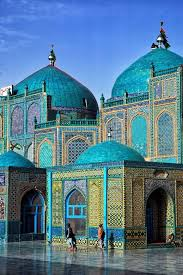
\includegraphics[width=1.06615in,height=1.6045in]{Images/image037.jpg}
    \caption{La mosquée bleue en Afghanistan est supposée être le lieu
du tombeau de ʿAlī. Rawze-i-Sharif (La Mosquée du Saint en référence à
Hazrat-e Ali Ibn Talib}
\end{marginfigure}


Par la suite, l'islam se structure autour de deux empires successifs,
rivaux~: l'empire omeyyade puis l'empire abbasside. Mais revenons à la
péninsule arabe à la naissance de l'islam et à son univers religieux.

\textbf{Conclusion}

Au départ de notre réflexion, une question~: comment connaître le
contexte culturel, religieux, politique de l'Arabie antéislamique~? Nous
remarquions que si nous disposons de sources musulmanes, elles ne
sauraient suffire, d'autant qu'elles participent d'une reconstruction
historique mettant en lumière le monde chaotique dans lequel se
trouvaient les tribus arabes avant la prédication de Muḥammad.

Cette difficulté épistémologique se retrouve dans l'histoire de l'islam
naissant et des premières dynasties. Or, il n'est pas possible de faire
l'histoire des premiers siècles sur la base des seules sources
musulmanes. Julius Wellhausen et Henri Lammens ont montré les failles de
l'histoire telle que la raconte l'historien al-Ṭabarī~: (nous l'avons
rencontré dans le commentaire de la bibliographie\ldots{} son traducteur
et analyste est Claude Gilliot). Je voudrais donner un exemple de ces
prismes au moment de la chute des Omeyyades en 750\sn{Sabatino
  Moscati, «~Le massacre des Umayyades dans l'histoire et dans les
  fragments poétiques~», Archiv Orientalni 18, 1950, p. 88-115.}.
L'histoire des Omeyyades, première dynastie de l'islam, est en effet
connue à partir de textes rédigés après l'arrivée des Abbassides. Or, si
le berceau des Omeyyades est la Syrie, les historiens écrivent dans
l'Irak abbasside à la fin du 9\textsuperscript{e} siècle après la
réinstallation du califat à Bagdad. Antoine Borrut montre qu'il fallait
réécrire l'histoire car «~les signes de continuité étaient devenus
inintelligibles~» après 150 ans de domination abbasside~:

«~Les épisodes successifs de la Révolution abbasside, de la guerre
civile entre les fils d'al-Rašīd, de la miḥna, du déplacement du califat
à Sāmarrā', de l'essor des militaires turcs, de l'assassinat
d'al-Mutawakkil et de la perte de la réalité du pouvoir par le calife,
suffisent amplement à expliquer cette perte de repères et le déficit de
cohérence dont souffrait alors l'histoire islamique~»\sn{Cité par
  Françoise Micheau, \emph{Les débuts de l'islam}, Paris, 2012, p. 28.}.

Il fallait donc rattacher directement les Abbassides à l'origine de
l'islam et faire tomber dans l'oubli la période omeyyade. Le massacre
des Omeyyades en 750 par les Abbassides est totalement omis dans
certains textes historiques. Al-Ṭabarī est pudique dans sa description
-- il faut dire qu'il fait désordre et pour fonder la légitimité
politique\ldots{} on peut faire mieux. Ibn Qutayba (m. 276/889) et
al-Mas`ūdī (m. 345/956) sont aussi peu prolixes. Les noms de ces trois
grands historiens ont déjà été mentionnés. Je redonne ici les dates avec
le calendrier hégirien\ldots{} alors que la première fois, je n'avais
mis que le calendrier grégorien\sn{Le calendrier hégirien est le
  calendrier musulman. L'année 0 est l'année de l'hégire, c'est-à-dire
  de la fuite de Muḥammad lorsqu'il quitte La Mecque. Nous sommes en 622
  dans le calendrier grégorien.}.

\textbf{La destruction des tombeaux des califes par les abbassides est
symptomatique de cette volonté de l'oubli. Mais malgré tout, les lieux
sont là et sont aujourd'hui redécouverts. Ils donnent de nouvelles
lumières sur les fondations de l'islam et l'histoire des premiers
siècles.}